% ==================================================
% FSE demo paper
%   4 pages in the ACM proceedings format, including all text, references and figures.
%
%   The paper must communicate clearly the following information to the audience:
%      1. the envisioned users
%      2. the software engineering challenge it proposes to address;
%      3. the methodology it implies for its users
%      4. the results of validation studies already conducted for mature tools, or the design of planned studies for early prototypes.
%   The paper must be accompanied by a short video (between 3 and 5 minutes long)
%
%   Paper    submission : June 29, 2018
%   Author   notification : July 16, 2018
%   Camera-ready deadline : July 30, 2018
% ==================================================
\documentclass[sigconf, review]{acmart}
%\pdfpagewidth=8.5in
%\pdfpageheight=11in
% !TEX root = ./1critics.tex
% -----------------------------------------------------------------
% package
% -----------------------------------------------------------------
\usepackage[numbers,sort&compress]{natbib}
\usepackage[utf8]{inputenc}
\usepackage[T1]{fontenc}
\usepackage{microtype}
\usepackage{color}
\usepackage{xcolor}
\usepackage{xspace}
%\usepackage[sort, space, compress]{cite}
\usepackage{algpseudocode}
%\usepackage[noend]{algorithmic}
\usepackage{amssymb}
\usepackage{pifont}
\usepackage{alltt}
\usepackage{framed,color}
\usepackage{soul}
\usepackage{multirow}
\usepackage{enumerate}
\usepackage{enumitem} % for better lists
\usepackage{colortbl} % for table highlighting
\makeatletter
\newif\if@restonecol
\makeatother
\let\algorithm\relax
\let\endalgorithm\relax
\usepackage[ruled,vlined]{algorithm2e}
%\usepackage[algo2e]{algorithm2e} 
\usepackage{stmaryrd} %for arrows
\usepackage{listings} %for code snippets
\usepackage{url}
\usepackage{pgfplots}
\usepackage{tikz}
\usepackage{balance}
\usepackage[listings]{tcolorbox}
\usepackage{soul}
\usepackage{graphicx}
% \usepackage[font=bf]{caption}
% \usepackage[font=bf]{subcaption}
\usepackage{qtree}
\usepackage{booktabs}
% \makeatletter  
%  \let\@copyrightspace\relax  
% \makeatother  
% -----------------------------------------------------------------
% color
% -----------------------------------------------------------------
\definecolor{darkBlue}{rgb}{0.000000,0.000000,0.545098}
\definecolor{darkGreen}{rgb}{0.000000,0.392157,0.000000}
\definecolor{DarkGray}{gray}{0.4}
\definecolor{javared}{rgb}{0.6,0,0} % for strings
\definecolor{javagreen}{rgb}{0.25,0.5,0.35} % comments
\definecolor{javapurple}{rgb}{0.5,0,0.35} % keywords
\definecolor{javadocblue}{rgb}{0.25,0.35,0.75} % javadoc
\definecolor{lightgray}{gray}{0.95}
\definecolor{shadecolor}{RGB}{150,150,150}
\definecolor{blueA}{RGB}{204,229,255}
\definecolor{redA}{RGB}{112,0, 0}
% -----------------------------------------------------------------
% abbreviations
% -----------------------------------------------------------------
\newcommand{\jinn}{Jinn\xspace}
\newcommand{\hidden}[1]{}
\newcommand{\xtc}{{\small\textsf{xtc}}}
\newcommand{\rats}{\textit{Rats!}}
\newcommand{\typical}{{\small\textsf{Typical}}}
\newcommand{\gctk}{GCTk\xspace}
\newcommand{\mmtk}{MMTk\xspace}
\newcommand{\jikes}{Jikes RVM\xspace}
\newcommand{\jikesrvm}{\jikes\xspace}
\newcommand{\jala}{Jalape\~{n}o\xspace}
\newcommand{\jalapeno}{Jalape\~{n}o\xspace}
\newcommand{\specjvm}{SPEC JVM\xspace}
\newcommand{\jess}{\textsf{\_202\_jess}\xspace}
\newcommand{\raytrace}{\textsf{\_205\_raytrace}\xspace}
\newcommand{\db}{\textsf{\_209\_db}\xspace}
\newcommand{\javac}{\textsf{\_213\_javac}\xspace}
\newcommand{\jack}{\textsf{\_228\_jack}\xspace}
\newcommand{\compress}{\textsf{\_201\_compress}\xspace}
\newcommand{\mpegaudio}{\textsf{\_222\_mpegaudio}\xspace}
\newcommand{\mtrt}{\textsf{\_227\_mtrt}\xspace}
\newcommand{\jbb}{\textsf{pseudojbb}\xspace}
\newcommand{\dacapo}{\textsf{DaCapo}\xspace}
\newcommand{\dacapover}{\textsf{DaCapo b.050224}\xspace}
\newcommand{\antlr}{\textsf{antlr}\xspace}
\newcommand{\bloat}{\textsf{bloat}\xspace}
\newcommand{\chart}{\textsf{chart}\xspace}
\newcommand{\eclipse}{\textsf{eclipse}\xspace}
\newcommand{\fop}{\textsf{fop}\xspace}
\newcommand{\hsqldb}{\textsf{hsqldb}\xspace}
\newcommand{\jython}{\textsf{jython}\xspace}
\newcommand{\luindex}{\textsf{luindex}\xspace}
\newcommand{\lusearch}{\textsf{lusearch}\xspace}
\newcommand{\pmd}{\textsf{pmd}\xspace}
\newcommand{\ps}{\textsf{ps}\xspace}
\newcommand{\xalan}{\textsf{xalan}\xspace}
\newcommand{\psfun}{\textsf{ps-fun}\xspace}
\newcommand{\ipsixql}{\textsf{ipsixql}\xspace}
\newcommand{\Ginseng}{{\sc Ginseng}\xspace}
\newcommand{\fixme} [1] {\textcolor{red}{{\it FIXME}: #1}}
\newcommand{\factfont}[1]{\scriptsize{{{#1}}}\normalsize}
\newcommand{\codefont}[1]{\footnotesize{\texttt{#1}}\normalsize}
\newcommand{\sydit}{\small \sc Sydit}
\newcommand{\reffinder}{\small \sc RefFinder}
\newcommand{\faulttracer}{\small \sc FaultTracer}
\newcommand{\iberry}{\small \sc Iberry}
\newcommand{\abs}[1]{\lvert#1\rvert}
\newcommand{\lase}{{\small {\sc Lase}}}
\newcommand{\genprog}{\small \sc GenProg}
\newcommand{\lsdiff}{\small \sc LSDiff}
\newcommand{\tool}{{\small{\sc{Soap}}}}
\newcommand{\critics}{{\tool}}
\newcommand{\maple}{{\small{\sc{Maple}}}}
\newcommand{\soa}{{\small{\sc{Soap}}}}

% -----------------------------------------------------------------
% misc
% -----------------------------------------------------------------
\newcommand{\addCode}{\textcolor{blue}}
\newcommand{\ax}{\textcolor{blue}{+}}
\newcommand{\delCode}{\textcolor{red}}
\newcommand{\dx}{\textcolor{red}{-}}
\newcommand{\susCode}{\textcolor{javagreen}}
\newcommand{\undoCode}{\textcolor{javagreen}{*}}
\newcommand{\myhref}[2]{\texttt{\scriptsize{\href{#1}{#2}}}}
\newcommand{\fix}[2]{\textbf{#1 asks:~\emph{ #2}}}
\newcommand{\pagemark}[1]{\textcolor{blue}{PAGE: {#1}}}
\newcommand{\todo}[1]{{\scriptsize{\textcolor{red}{{\bf TODO}: {#1}}}}}
\newcommand{\tianyi}[1]{#1}
\newcommand{\old}[1]{\textcolor{red}{{}}}
\newcommand{\did}[1]{{\textcolor{red}{{#1}}}}
\newcommand{\oo}[1]{{\scriptsize{\textcolor{red}{{\bf*} {#1}}}}}
\newcommand{\ignore}[1]{}
\newcommand{\mccenter}[1]{\multicolumn{1}{c|}{#1}}
\newcommand{\m}[1]{\textcolor{blue}{#1}}
\newcommand{\selectbox}[1]{\par\colorbox{blueA}
{\parbox{\dimexpr\textwidth-17\fboxsep\relax}{#1}}}
\newcommand{\hilight}[1]{\colorbox{blueA}{#1}}
\newcommand{\hilightR}[1]{\colorbox{red}{\textcolor{yellow}{#1}}}
\newcommand{\fn}[1]{\footnote{\scriptsize{#1}}}

\newcommand{\ttt}[1]{\tt\small{#1}}
\newcommand{\tttt}[1]{\tt\scriptsize{#1}}


% -----------------------------------------------------------------
% indent dense
% -----------------------------------------------------------------
\def\denseitems 
{
  \itemsep1pt plus1pt minus1pt
  \parsep0pt plus0pt
  \parskip0pt\topsep0pt
}
% -----------------------------------------------------------------
% 
% -----------------------------------------------------------------
\chardef\oc=`\{
\chardef\cc=`\}
\chardef\us=`\_
\def\Note#1{\emph{\textbf{\small $<$#1$>$}}}
% -----------------------------------------------------------------
% 
% -----------------------------------------------------------------
\newcommand{\cmark}{\ding{51}}%
\newcommand*{\smalltt}[1]{\texttt{\small{}#1}}
% ===============================================
% MyJavaStyle
% ===============================================
\lstdefinestyle{MyJavaStyle} {
  language=Java,
  frame=lines,
  xleftmargin=15pt, 
  stepnumber=1, 
  numbers=left, 
  numbersep=5pt,
  numberstyle=\tiny\color[gray]{0.777}, 
  belowcaptionskip=\bigskipamount,
  captionpos=b, 
  escapeinside={*'}{'*},
  tabsize=5,
  emphstyle={\bf},
  basicstyle=\footnotesize\ttfamily,
  keywordstyle=\color{black}\bfseries,
  stringstyle=\color{black},
  commentstyle=\color{black},
  morecomment=[s][\color{black}]{/**}{*/},
  showspaces=false,
  columns=flexible,
  showstringspaces=false,
  morecomment=[l]{//},
  tabsize=2,
  morekeywords={, Package,Invariant,Class,Method,Field,Where,in,Assert,ToLc,Split,Msg,Immutable,<<<,eq,neq,not,has,Assert,AssertExists,Attribute,Uc,Lc,},
  breaklines=true
}
% ===============================================
% MyJavaSmallStyle
% ===============================================
\lstdefinestyle{MyJavaSmallStyle} {
  language=Java,
  frame=none,
  xleftmargin=15pt, 
  stepnumber=1, 
  numbers=left, 
  numbersep=5pt,
  numberstyle=\tiny\color[gray]{0.777}, 
  belowcaptionskip=\bigskipamount,
  captionpos=b, 
  escapeinside={*'}{'*},
  tabsize=5,
  emphstyle={\bf},
  basicstyle=\scriptsize\ttfamily,
  keywordstyle=\color{javapurple}\bfseries,
  stringstyle=\color{javared},
  commentstyle=\color{javagreen},
  morecomment=[s][\color{javadocblue}]{/**}{*/},
  showspaces=false,
  columns=flexible,
  showstringspaces=false,
  morecomment=[l]{//},
  tabsize=2,
  morekeywords={, Package,Invariant,Class,Method,Field,Where,in,Assert,ToLc,Split,Msg,Immutable,<<<,eq,neq,not,has,Assert,AssertExists,Attribute,Uc,Lc,},
  breaklines=true
}
% ===============================================
% MyJavaNonColorStyle
% ===============================================
\lstdefinestyle{MyJavaNonColorStyle} {
  language=Java,
  frame=lines,
  xleftmargin=15pt, 
  stepnumber=1, 
  numbers=left, 
  numbersep=5pt,
  numberstyle=\tiny\color[gray]{0.3}, 
  belowcaptionskip=\bigskipamount,
  captionpos=b, 
  escapeinside={*'}{'*},
  tabsize=5,
  emphstyle={\bf},
  basicstyle=\scriptsize\ttfamily,
  keywordstyle=\color{black}\bfseries,
  stringstyle=\color{black},
  commentstyle=\color{black},
  morecomment=[s][\color{black}]{/**}{*/},
  showspaces=false,
  columns=flexible,
  showstringspaces=false,
  morecomment=[l]{//},
  tabsize=2,
  morekeywords={, Package,Invariant,Class,Method,Field,Where,in,Assert,ToLc,Split,Msg,Immutable,<<<,eq,neq,not,has,Assert,AssertExists,Attribute,Uc,Lc,},
  breaklines=true
}
% ===============================================
% Global Setting: MyJavaStyle
% ===============================================
\lstset{style=MyJavaStyle}
% ===============================================

% ===============================================
%    URL style
% ===============================================
%% Define a new 'leo' style for the package that will use a smaller font.
%% Now actually use the newly defined style.
\urlstyle{leo}
% ===============================================
% -----------------------------------------------------------------
% spacing
% -----------------------------------------------------------------
%\clubpenalty 10000
%\widowpenalty 10000
%\def\topfraction{0.9}
%\def\bottomfraction{0.9}
%\def\textfraction{0.1}
%\newcommand{\singlespace}{\renewcommand{\baselinestretch}{1.00}\small\normalsize}
%\newcommand{\doublespace}{\renewcommand{\baselinestretch}{1.5}\small\normalsize}
%\newcommand{\tight}{\renewcommand{\baselinestretch}{1.10}\small\normalsize}
%\renewcommand{\subfigbottomskip}{0.25ex}
%\renewcommand{\subfigcapskip}{0ex}
% -----------------------------------------------------------------
% margins
% -----------------------------------------------------------------
%\topmargin -0.1truein
%\textheight 9truein
%\oddsidemargin .25truein
%\evensidemargin .25truein
%\textwidth 6truein
% -----------------------------------------------------------------
% sectioning commands See Latex Companion, pp24-30 for details
% -----------------------------------------------------------------
%\setcounter{secnumdepth}{2}
%\makeatletter
%%\parskip=0pt
%\renewcommand\section{\@startsection{section}
%        {1}%    level
%        {\z@}%  indent
%        {-2.5ex}% beforeskip
%        {.5ex}% afterskip
%        {\normalfont\normalsize\bfseries\parskip=0pt}}% style
%\renewcommand\subsection{\@startsection{subsection}
%        {2}%    level
%        {\z@}%  indent
%        {-1ex}% beforeskip
%        {.2ex}% afterskip
%        {\normalfont\normalsize\bfseries\parskip=0pt}}
%\renewcommand\subsubsection{\@startsection{subsubsection}%
%        {3}%    level
%        {0em}%  indent
%        {1ex}%  beforeskip
%        {-.5em}% afterskip
%        {\normalfont\normalsize\bfseries\parskip=0pt}}% style
%% The following will generate compact para headings
%\renewcommand\paragraph{\@startsection{paragraph}%
%        {4}%    level
%        {0em}%  indent
%        {.5ex}%  beforeskip
%        {-.5em}% afterskip
%        {\normalfont\normalsize\bfseries\parskip=0pt}}% style
%\setlength\partopsep{0pt}
%\setlength\parskip{1.5ex}
%\setlength\parindent{0pt}
%\makeatother
% -----------------------------------------------------------------
% 
% -----------------------------------------------------------------
%\newenvironment{narrow}[1][\parindent]{%
%  \list{}{%
%    \setlength{\leftmargin}{#1}%
%    \setlength{\rightmargin}{#1}%
%  }%
%  \item\relax%
%}{%
%  \endlist%
%}
% -----------------------------------------------------------------
% jinnconstraint
% -----------------------------------------------------------------
%\newcommand{\jinnconstraint}[4]{%
%\centerline{  
%\vspace*{1ex}\noindent{%
%    %\framebox{\begin{minipage}{0.973\columnwidth}%
%    {\begin{minipage}{0.9\columnwidth}%
%        \vspace*{4pt}\centerline{\hspace*{-1em}\rule{40em}{0.4pt}}
%        \begin{list}{}{
%            \setlength{\topsep}{0pt}
%            \setlength{\parsep}{0pt}
%          }
%        \item[{\bf{#1}}:]    {#2}
%        %\hspace*{-1em}\rule{20em}{0.4pt}
%        \item[\emph{State}:] \hspace*{3pt}{#3}
%        \item[\emph{Check}:] {#4}
%        \end{list}%
%        \vspace*{-6pt}\centerline{\hspace*{-1em}\rule{40em}{0.4pt}}
%              \end{minipage}}}}}
% -----------------------------------------------------------------
% listings config
% -----------------------------------------------------------------


\setcopyright{rightsretained}
\acmConference[ESEC/FSE 2018]{The 26th ACM Joint European Software Engineering Conference and Symposium on the Foundations of Software Engineering}{4--9 November, 2018}{Lake Buena Vista, Florida, United States}

% correct bad hyphenation here
\hyphenation{op-tical net-works semi-conduc-tor}

\begin{document}

\title{Augmenting Stack Overflow with API Usage Patterns Mined from GitHub}

\author{Anastasia Reinhardt\textsuperscript{1}\footnotemark\,\,Tianyi Zhang\textsuperscript{2}\,\,Mihir Mathur\textsuperscript{2}\,\,Miryung Kim\textsuperscript{2}}
\authornote{Work done as an intern at University of California, Los Angeles.}
\affiliation{\textsuperscript{1}George Fox University}
\affiliation{\textsuperscript{2}University of California, Los Angeles}
\affiliation{areinhardt14@georgefox.edu, \{tianyi.zhang, miryung\}@cs.ucla.edu, mihirmathur@ucla.edu}

\renewcommand{\authors}{Anastasia Reinhart, Tianyi Zhang, Mihir Mathur, and Miryung Kim}
\renewcommand{\shortauthors}{Anastasia Reinhart, Tianyi Zhang, Mihir Mathur, and Miryung Kim}


%\author{Anastasia Reinhardt}
%\affiliation{George Fox University}
%\email{areinhardt14@georgefox.edu}
%
%\author{Tianyi Zhang, Mihir Mathur, Miryung Kim}
%\affiliation{University of California, Los Angeles}
%\email{tianyi.zhang@cs.ucla.edu}
%
%\author{Mihir Mathur}
%\affiliation{University of California, Los Angeles}
%\email{mihirmathur@ucla.edu}
%
%\author{Miryung Kim}
%\affiliation{University of California, Los Angeles}
%\email{miryung@cs.ucla.edu}


% ==================================================
% abstract
% ==================================================
\begin{abstract}
	Programmers often consult Q\&A websites such as Stack Overflow (SO) to learn new APIs. However, online code snippets are not always complete or reliable in terms of API usage. To assess online code snippets, we build a Chrome extension, {\tool} that detects API usage violations in SO posts using API usage patterns mined from 380K GitHub projects. It quantifies how many GitHub examples follow common API usage and illustrates how to remedy the detected violation in a given SO snippet. With {\tool}, programmers can easily identify the pitfalls of a given SO snippet and learn how much it deviates from common API usage patterns in GitHub. The demo video is at~\small{\url{https://youtu.be/WOnN-wQZsH0}}.
\end{abstract}


\begin{CCSXML}
<ccs2012>
<concept>
<concept_id>10011007.10010940.10011003.10011004</concept_id>
<concept_desc>Software and its engineering~Software reliability</concept_desc>
<concept_significance>300</concept_significance>
</concept>
<concept>
<concept_id>10011007.10011074.10011134</concept_id>
<concept_desc>Software and its engineering~Collaboration in software development</concept_desc>
<concept_significance>300</concept_significance>
</concept>
<concept>
<concept_id>10011007.10011006.10011066.10011069</concept_id>
<concept_desc>Software and its engineering~Integrated and visual development environments</concept_desc>
<concept_significance>300</concept_significance>
</concept>
</ccs2012>
\end{CCSXML}

\ccsdesc[300]{Software and its engineering~Software reliability}
\ccsdesc[300]{Software and its engineering~Collaboration in software development}
\ccsdesc[300]{Software and its engineering~Integrated and visual development environments}

\keywords{online Q\&A forum, API usage pattern, code assessment}  

\maketitle

% ==================================================
% Introduction
% ==================================================
% ==============================================
% !TEX root = ./critics.tex
% ==============================================
% ==============================================
\section{Introduction}
\label{sec:intro}
% ==============================================
% Problem
Programmers often search for online code examples to learn new APIs. A case study at Google shows that developers issue an average of 12 code search queries per weekday~\cite{sadowski2015developers}. Stack Overflow (SO) is a popular Q\&A website that programmers often consult. In July 2017, Stack Overflow has accumulated more than 22 million answers, many of which contain code examples to demonstrate the solution for a particular programming question. However, SO examples are not always complete or reliable, which can be misleading and potentially dangerous when programmers follow the same example to complete a client program. Our previous study shows that over 50\% of 31,801 SO posts contain API misuse that could produce symptoms of program crashes and resource leaks if reused in a target system.\todo{cite our API misuse study on Stack Overflow} %Neglecting to close an input stream, for example, could lead to data leakage or generally unreliable code. 

%system flow diagram of the UI
\begin{figure}
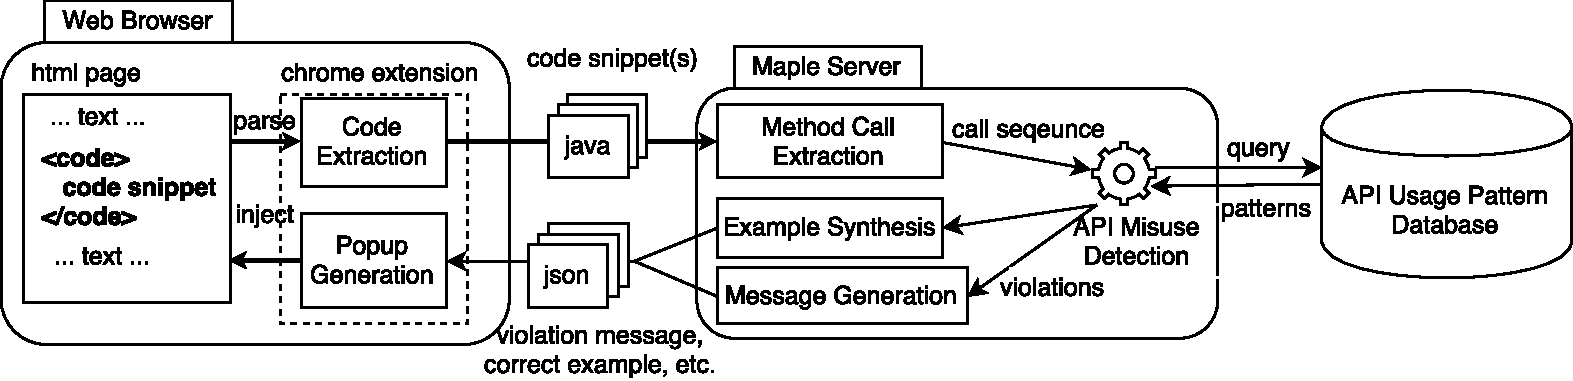
\includegraphics[width=0.48\textwidth]{maple-extension-v1.pdf}
\vspace{.1in}
\caption{An overview of {\soa}'s architecture}
\label{fig:arch}
\end{figure}

% Solution
To assess online code examples, this paper presents {\soa}, an interactive approach that augments Stack Overflow with code idioms learned from GitHub and alerts programmers about the potential violations in a code example. {\soa} leverges a scalable API usage mining technique to learn three types of API-related idioms---temporal ordering, guard conditions, and exception handling of API calls---from over 7 million GitHub projects. Our insight is that commonly practiced idioms in massive code corpora may represent a desirable pattern that a programmer can use to trust and enhance code examples on Stack Overflow. 

Given an SO example, {\soa} first extracts the sequence of API calls with corresponding control constructs and guard conditions. {\soa} then contrasts the sequence with commonly practiced idioms in GitHub and highlights code regions that violate the idioms. To help users better understand the violations, {\soa} further generates descriptive warning messages and also contextualizes a violated idiom by synthesizing a fixed example. Mining code idioms to detect API usage violations often suffers from reporting false alarms, since mined idioms may not be inclusive and fit all use scenarios of an API~\cite{liang2016antminer}. To mitigate this issue, {\soa} allows users to upvote or downvote a violation based on its applicability and usefulness to an SO example. {\soa} filters a code idiom when multiple users flag it as unhelpful to assess an example. To help developers build confidence on a code idiom, {\soa} shows how many GitHub developers also follow the idiom as well as how many other users like or dislike this idiom.

A user of {\soa} would benefit from the addition of quantitative examples from compiled GitHub resources to the code examples she encounters on Stack Overflow. This will not only combat programming issues stemming from the use of incomplete or unreliable SO code examples, but will also be an aid for users learning a new API. By enhancing examples already found in Stack Overflow, a user can trust that she will learn common and reliable usage patterns for a given API.
%A user of this tool would benefit from not needing to cross-reference multiple sites for proper API usage reference, and will be able to continue using Stack Overflow to learn APIs with the added advantage of seeing which usage patterns a post may have left out of its explanation. This could result in more complete, reliable code with minimal added time or effort on the part of the programmer.\todo{The description here does not sound very appealing. Can you rework this paragraph?} 

This paper's main contribution is to describe the features of {\soa} from a user's perspective. In order to give programmers access to {\soa}, the front-end of {\soa} is implemented as a Chrome extension that users can easily download and install.\todo{add a url to download our tool} The detailed algorithm and study are described in our separate technical report.\todo{cite our API misuse study}

%input{fig_motiExample}
%\input{fig_UI}


% ==================================================
% Motivating Example and Tool Features
% ==================================================
% ==============================================
\section{Demonstration Scenario}
\label{sec:motivation}

% ==============================================
%\begin{figure*}
%\centering
%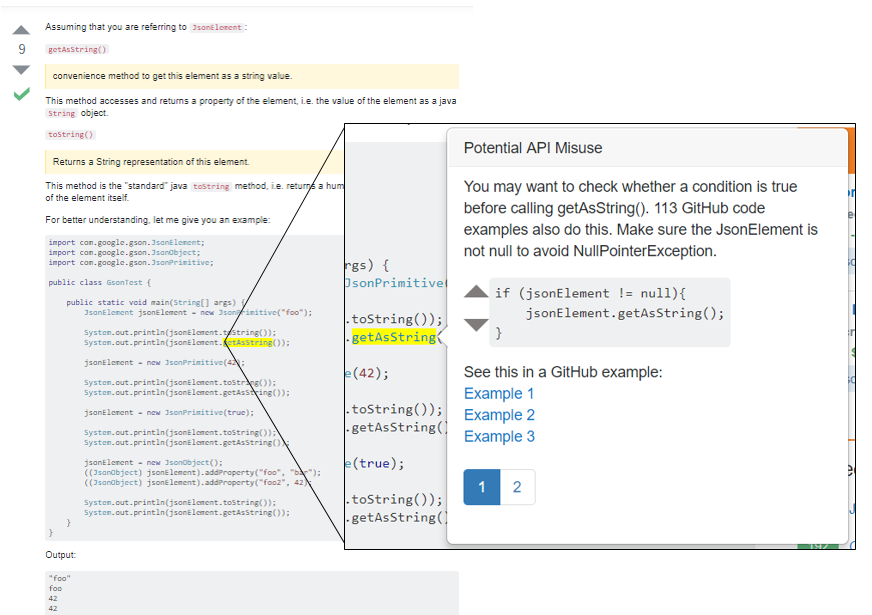
\includegraphics[width=0.6\textwidth]{json_ex1_context.PNG}
%  \vspace{.1in}
%  \caption{A code snippet that does not properly check {\tt JsonElement.getAsString}.\protect\footnotemark}
%  \label{fig:so_example}
%\end{figure*}
%
%\begin{figure*}[t!]
%\centering
%  \begin{subfigure}[t]{0.48\textwidth}
%  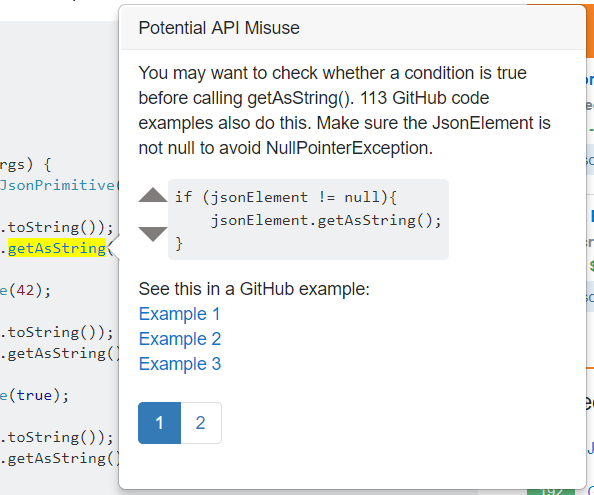
\includegraphics[width=\textwidth, height=6cm]{json_ex2.PNG}
%  \caption{A page describing a way to avoid a {\tt NullPointerException} by checking whether the {\tt JsonElement} object is null. \todo{should I still include this figure when it's sort of subsumed by Figure~\ref{fig:so_example}?}} 
%  \label{fig:page1}
%  \end{subfigure}
%  \hspace{0.02\textwidth}
%  \begin{subfigure}[t]{0.48\textwidth}
%  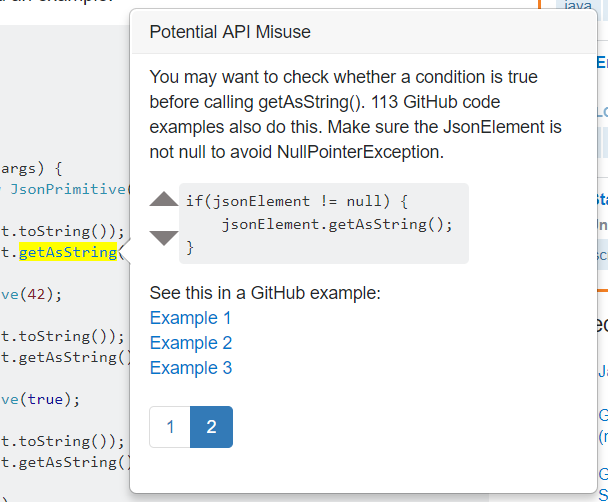
\includegraphics[width=\textwidth, height=6cm]{json_ex3.PNG}
%  \caption{A page describing a way to avoid a {\tt ClassCastException} by checking whether the {\tt JsonElement} object is a primitive.}
%  \label{fig:page2}
%  \end{subfigure}
%  \hfill
%  \vspace{0.02\textwidth}
%\caption{The two pages of a popup generated on {\tt JsonElement.getAsString}.\todo{Can we also show how many users like or dislike the violations in the popup window? Since we don't have any real users, maybe we need to create some artificial numbers for the demonstration purpose.}}
%\label{fig:features}
%\end{figure*}

Suppose Alice wants to read attribute values from a {\ttt JSON} message using Google's Gson library. Alice searches online and finds a related Stack Overflow post with an illustrative code example, as shown in Figure~\ref{fig:screenshot}.\footnote{\url{https://stackoverflow.com/questions/29860000}} Though this post is accepted as a correct answer, it does not properly use the {\ttt JsonElement.getAsString} method, which gets the {\ttt string} value of a {\ttt JSON} element. For example, if the requested attribute does not exist in the {\ttt JSON} message, the preceding API call, {\ttt JsonObject.get} will return {\ttt null}, which consequently leads to {\ttt NullPointException} when calling {\ttt getAsString} on the returned object. If Alice puts too much trust on this example of the SO post, she may inadvertently follow an unreliable solution, which might lead to runtime errors in some corner cases. 

Alice cannot easily recognize the potential limitation of the given SO post, unless she manually investigates other similar code examples. {\tool} frees Alice from this manual investigation labor by contrasting a Stack Overflow post with common API usage patterns mined from over 380K GitHub repositories. {\tool} then highlights the potential API usage violations in the Stack Overflow post. When Alice clicks on a highlighted API call, {\tool} generates a pop-up window with detailed descriptions about the API usage violation, as shown in Figure~\ref{fig:screenshot}.

{\bf API misuse description.} To help Alice understand a detected API usage violation, {\tool} translates the violation to a  natural language description (\ding{172} in Figure~\ref{fig:screenshot}). From the warning message, Alice learns that she should check whether the {\ttt JsonElement} object is {\ttt null} before calling {\ttt getAsString}. {\tool} also displays a message that 119 GitHub examples also follow this usage pattern. Such quantification can provide additional evidence about how many real-world examples are different from the given SO snippet.

\begin{figure}
\centering
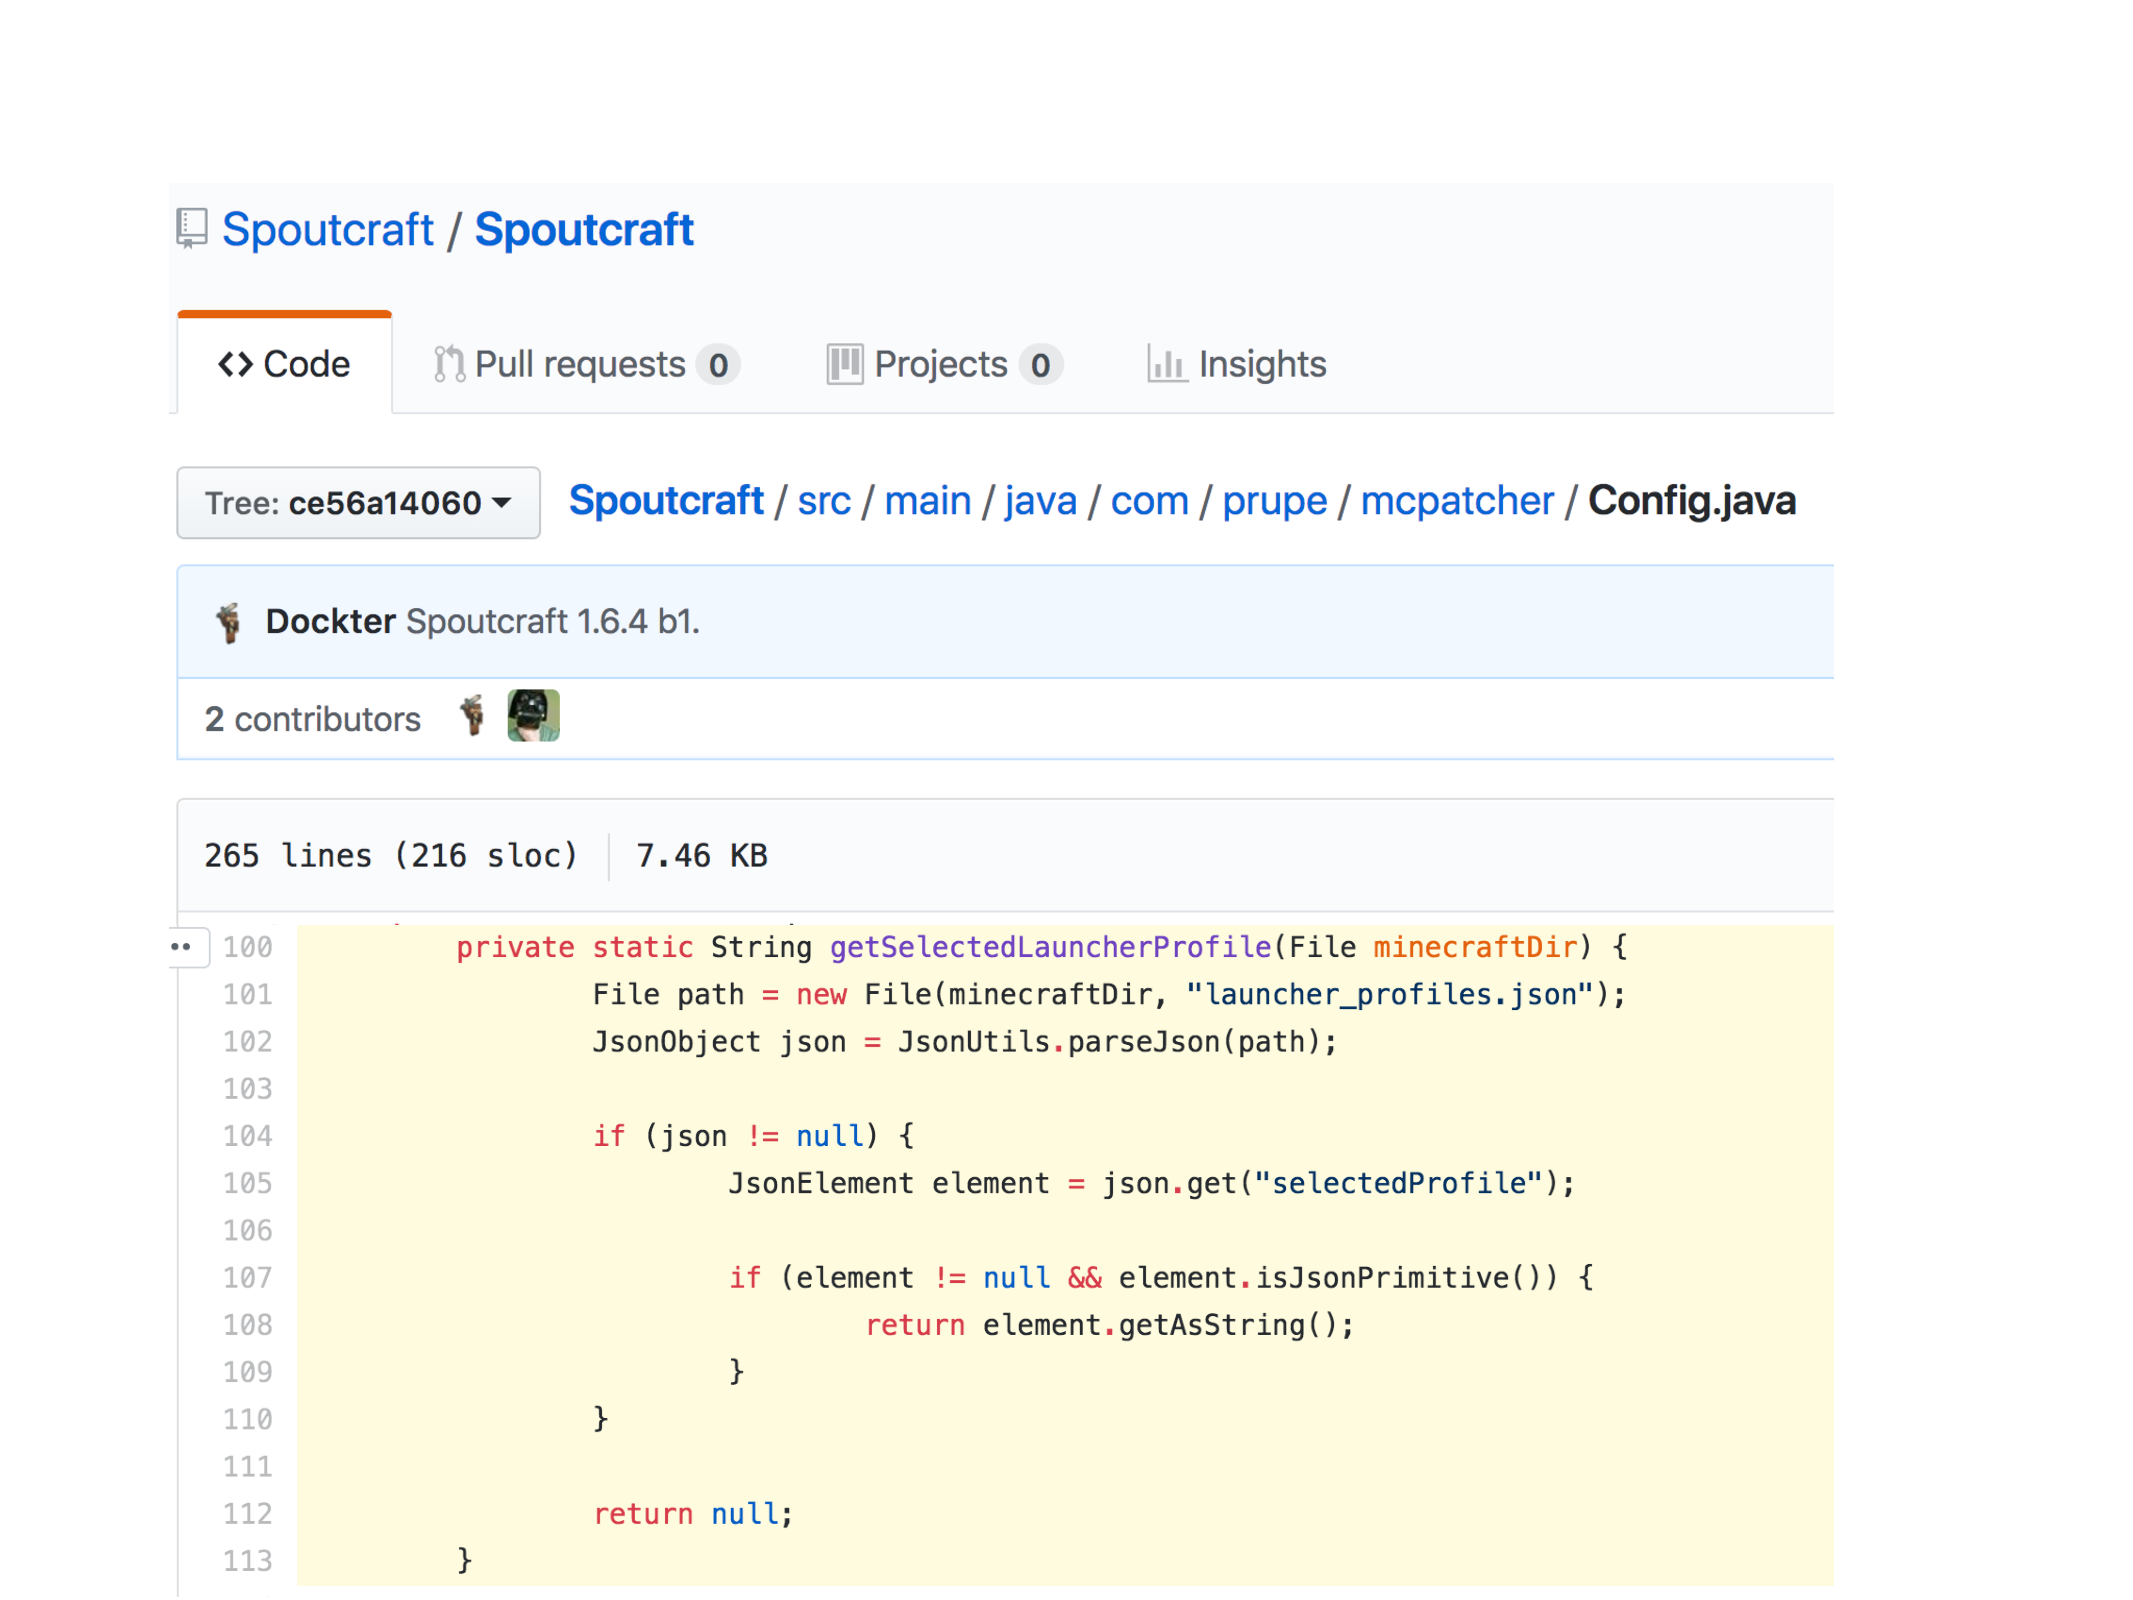
\includegraphics[width=0.48\textwidth]{github-example-v3.pdf}
%\caption{{\tool} will redirect a programmer to a concrete code example from GitHub that follows a correct API usage pattern, when she clicks on a GitHub example link in the pop-up window.\protect\footnotemark}
\caption{A programmer can view a concrete code example from GitHub that follows a correct API usage pattern, when clicking on a GitHub example link in the pop-up window.\protect\footnotemark}
  \label{fig:github}
\end{figure}

\footnotetext{\url{https://goo.gl/YHo1UM}}

{\bf Fix suggestion.} {\tool} further sketches how to correct the violation in the original SO post, as shown in \ding{174} in Figure~\ref{fig:screenshot}. This fix is an embodiment of the correct API usage pattern in the context of the SO post. To reduce the gap between the fix and the original post, {\tool} reuses the same variable names in the original SO posts to generate a suggestion with improved API usage. For example, the {\ttt JsonElement} variable in the generated example is named as the same variable, {\ttt match\_number} in the original post.

{\bf Linking GitHub examples.} To help Alice understand how the same API method is used in real-world projects, {\tool} provides several GitHub examples that follow the suggested API usage pattern (\ding{176} in Figure~\ref{fig:screenshot}). Alice is curious about how others use {\ttt JsonElement.getAsString}. When she clicks on the link of the first GitHub example, {\tool} redirects Alice to a GitHub page and automatically scrolls down to the Java method where {\ttt JsonElement.getAsString} is called, as shown in Figure~\ref{fig:github}. Compared with the simplified SO example in Figure~\ref{fig:screenshot}, this GitHub code is more carefully constructed with multiple {\ttt if} checks. For example, it not only checks whether the {\ttt JsonElement} object is {\ttt null}, but also checks whether it is a primitive type to avoid {\ttt ClassCastException} before calling {\ttt getAsString}. By providing the traceability to concrete code examples in GitHub, Alice could gain a more comprehensive view of correct API usage in production code, which may not be illustrated in simplified code examples in Stack Overflow. 

{\bf User feedback.} After investigating the concrete example in GitHub, Alice finds it necessary to perform a {\ttt null} check. She upvotes the pattern by clicking on the ``thumbs-up'' button to notify other users that this detected violation is helpful (\ding{175} in Figure~\ref{fig:screenshot}). Alice also finds that her decision resonates with the majority of {\tool} users, since nine users also upvoted this violation.

\begin{figure}
\centering
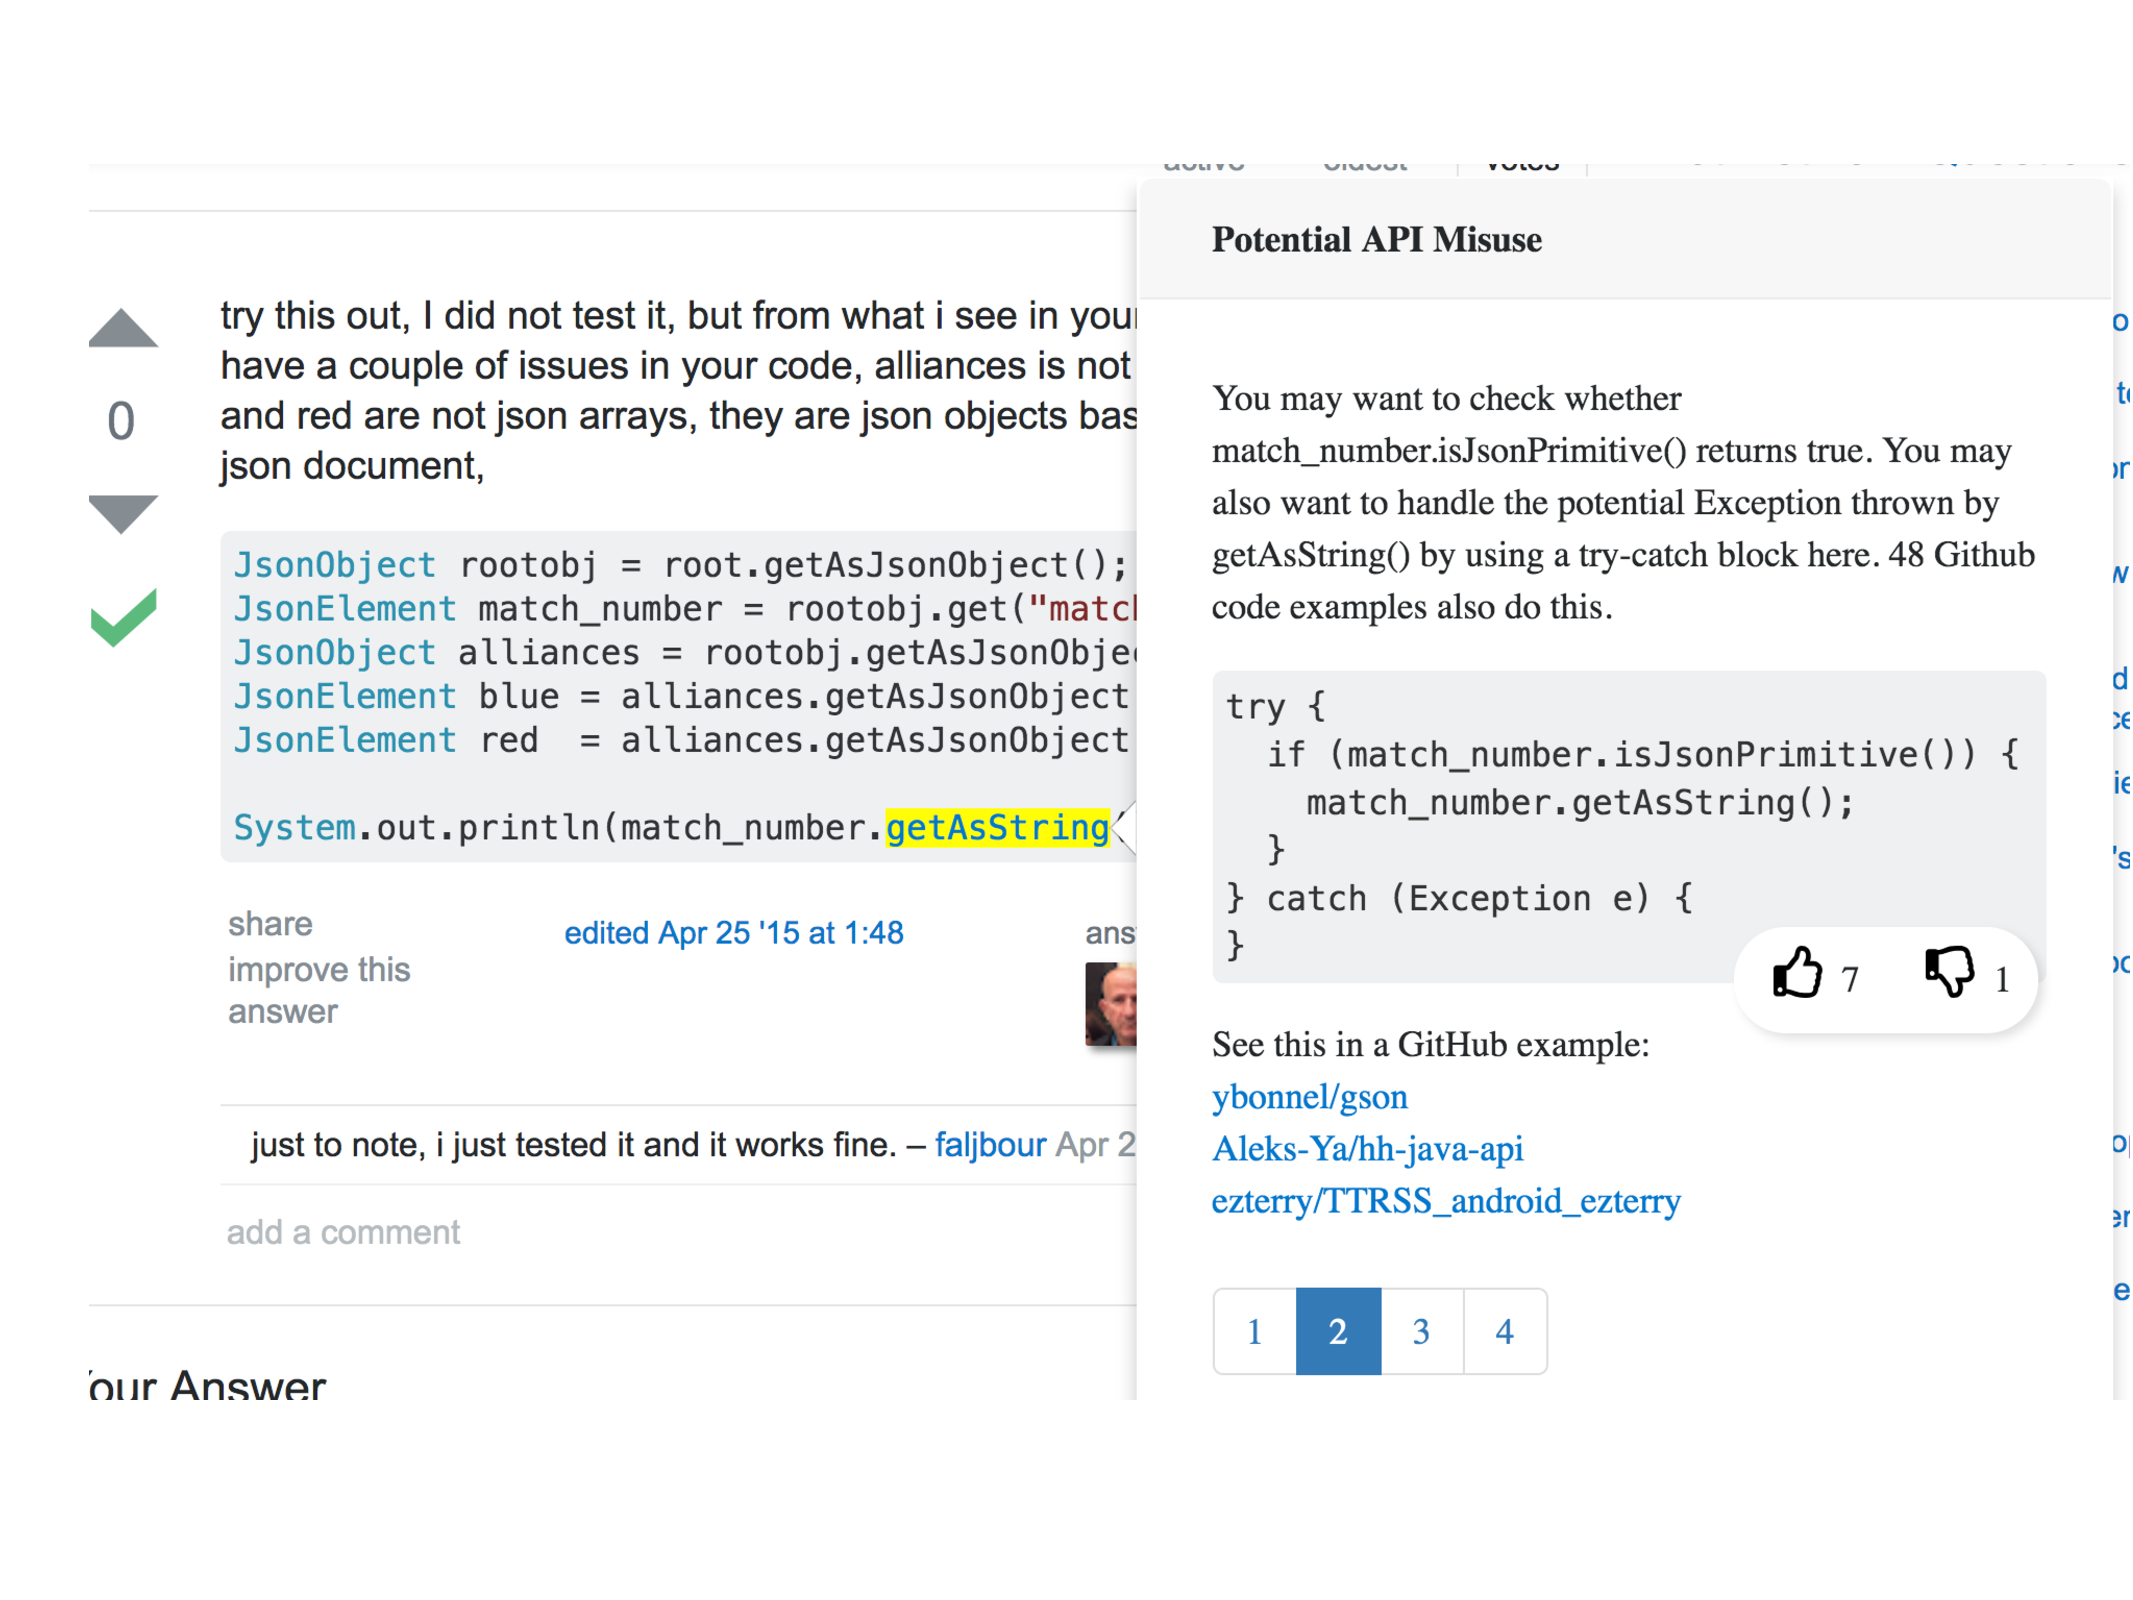
\includegraphics[width=0.48\textwidth]{examplecheck-page2.pdf}
  \caption{Another API usage warning that reminds programmers to check whether the {\ttt JsonElement} object represents a {\ttt JSON} primitive value by calling {\ttt isJsonPrimitive}. It also suggests to catch potential exceptions thrown by {\ttt getAsString}.}
  \label{fig:screenshot2}
\end{figure}

{\bf Multiple API usage violations.} If a method call in a SO post violates multiple API usage patterns, {\tool} displays them in separate pages in a pop-up window. These pages are first ranked by the vote score (i.e., upvotes minus downvotes) of each violated pattern, and then by the number of GitHub examples that support a pattern if two patterns have the same vote score. As shown in \ding{177} in Figure~\ref{fig:screenshot}, the method call, {\ttt getAsString} violates four API usage patterns. Figure~\ref{fig:screenshot2} shows the second violated pattern and suggests Alice to check whether the {\ttt JsonElement} object represents a {\ttt JSON} primitive value before calling {\ttt getAsString}. Otherwise, {\ttt getAsString} will throw {\ttt ClassCastException}. {\tool} also suggests Alice to wrap {\ttt getAsString} with a {\ttt try-catch} block to handle potential exceptions. This pattern is supported by 48 GitHub examples.

%\begin{figure*}[t!]
%\centering
%  \begin{subfigure}[t]{0.48\textwidth}
%  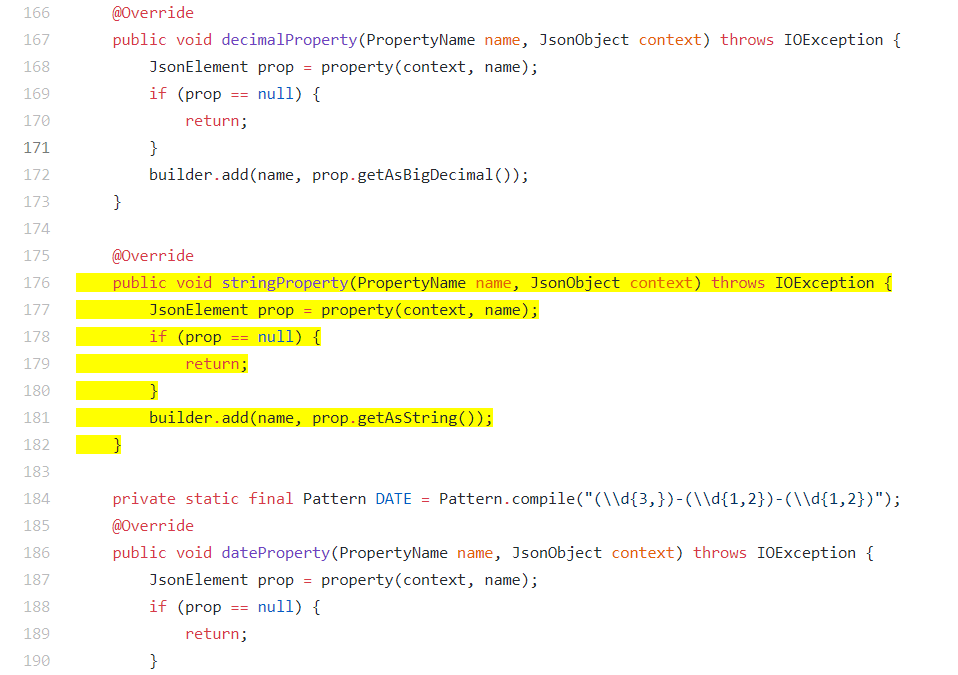
\includegraphics[width=\textwidth]{json_null_gh2_context.PNG}
%  \caption{The second GitHub example for Figure~\ref{fig:page1} in the context of its GitHub file.\protect\footnotemark} 
%  \vspace{.1in}
%  \label{fig:github1}
%  \end{subfigure}
%  \hfill
%  \begin{subfigure}[t]{0.48\textwidth}
%  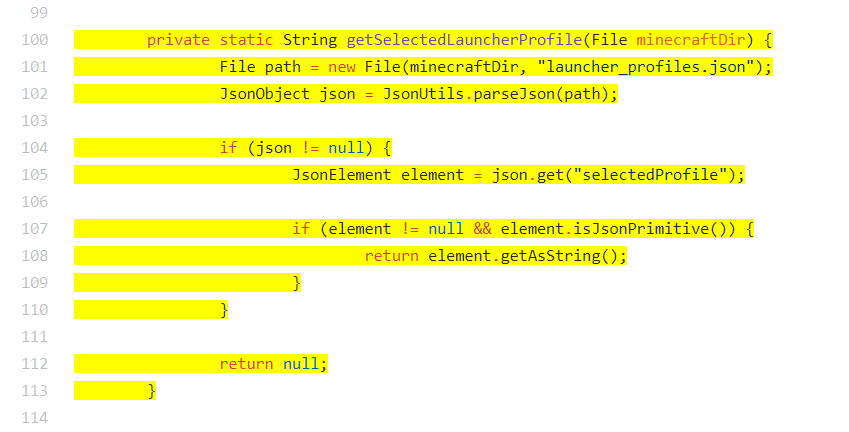
\includegraphics[width=\textwidth]{json_primitive_gh1.PNG}
%  \caption{The first GitHub example for Figure~\ref{fig:page2}.\protect\footnotemark}
%  \vspace{.1in}
%  \label{fig:github2}
%  \end{subfigure}
%  \hfill
%\caption{The GitHub examples redirected to from the links provided in the popup, highlighted by the Chrome extension.\todo{The snapshot only shows the highlighted code. Is there a better way to give paper reviewers some context that the highlighted code is from GitHub and that the code is selectively highlighted by our tool instead of by GitHub?}}
%\label{fig:github_examples}
%\end{figure*}

%\begin{figure}
%\centering
%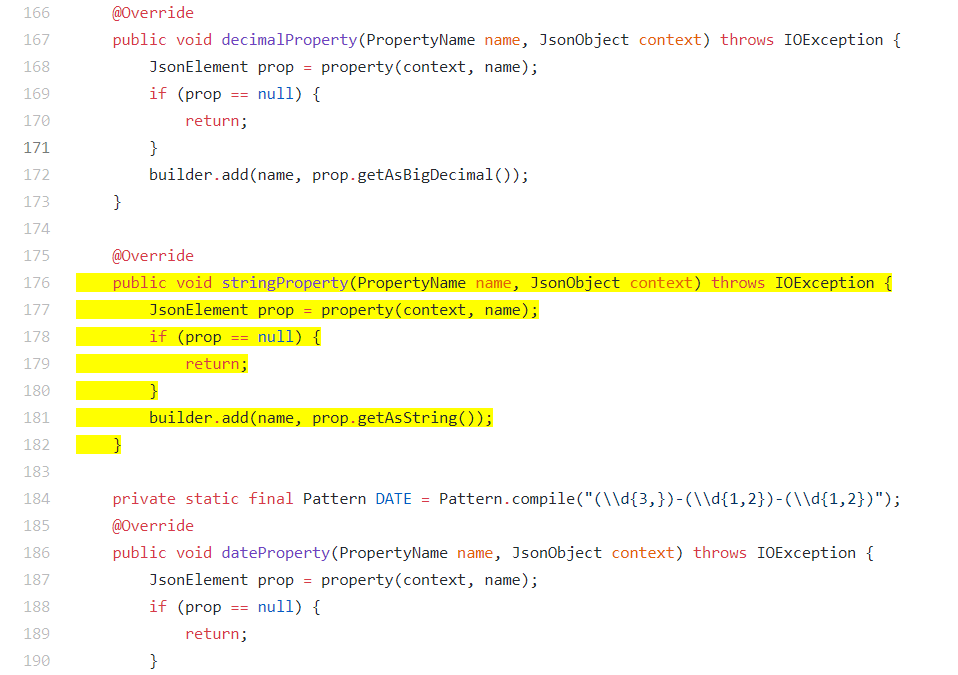
\includegraphics[width=0.48\textwidth]{json_null_gh2_context.PNG}
  %\caption{The GitHub example that a link from Figure~\ref{fig:page1} redirects to, highlighted by the Chrome extension.\protect\footnotemark} 
  %\label{fig:github_examples}
%\end{figure}

%https://github.com/asakusafw/asakusafw/blob/cad94753128bd3168e23c0539cc55c7e5a653dbd/asakusa-test-data-provider/src/main/java/com/asakusafw/testdriver/json/JsonObjectDriver.java
%\footnotetext{http://tinyurl.com/JsonObjectDriver}

%https://github.com/Spoutcraft/Spoutcraft/blob/5cbbc2b07edaf4194a36130a7e74321e5b30ace0/src/main/java/com/prupe/mcpatcher/Config.java
%\footnotetext{http://tinyurl.com/SpoutcraftConfig}


% ==================================================
% Approach
% ==================================================
\section{Implementation}
\label{sec:implementation}

This section describes the implementation details of {\tool}. Figure~\ref{fig:arch} shows the architecture of {\tool}.  When a user loads a Stack Overflow page in the Chrome browser, the Chrome extension extracts code snippets within {\ttt <code>} tags in answer posts, and sends them to the back-end server in a {\ttt JSON} message. The back end then detects API usage violations in a snippet and synthesizes violation descriptions and fixes. For each misused method call in a snippet, the Chrome extension generates a pop-up window using the Bootstrap popover plug-in\footnote{\url{https://www.w3schools.com/bootstrap/bootstrap_popover.asp}} to visualize the violation information received from the server.


\begin{table*}[!th]
\centering
\resizebox{\textwidth}{!}{%
\begin{tabular}{|l|l|l|}
\hline
\multicolumn{1}{|c|}{\sf Violation Type}    & \multicolumn{1}{c|}{\sf Description Template}                                                                                                  & \multicolumn{1}{c|}{\sf Example Warning Message}                                                                                                  \\ \hline
Missing/Incorrect Order of API calls & You may want to call {\bf \textless?\textgreater} {\bf \textless before/after\textgreater} calling {\bf \textless?\textgreater}                   & \begin{tabular}[c]{@{}l@{}}You may want to call {\ttt TypedArray.recycle()} after calling\\ {\ttt TypedArray.getString()}.  [\colorbox{lightgray}{\href{https://stackoverflow.com/questions/35784171}{35784171}}]\end{tabular}                                    \\ \hline
Missing Control Constructs              & You may want to call the API method {\bf \textless?\textgreater} in {\bf \textless?\textgreater}                           & \begin{tabular}[c]{@{}l@{}}You may want to call {\ttt Cursor.close()} in a finally block. [\colorbox{lightgray}{\href{https://stackoverflow.com/questions/31427468}{31427468}}]\end{tabular}                                                            \\ \hline
Missing Try-Catch                       & \begin{tabular}[c]{@{}l@{}} You may want to handle the potential {\bf \textless?\textgreater} exception thrown\\ by {\bf \textless?\textgreater} using a try-catch block\end{tabular} & \begin{tabular}[c]{@{}l@{}}You may want to handle the potential {\ttt SQLException} thrown by\\ {\ttt PreparedStatement.setString()} using a try-catch block. [\colorbox{lightgray}{\href{https://stackoverflow.com/questions/11183042}{11183042}}]\end{tabular} \\ \hline
Incorrect Guard Conditions              & You may want to check whether {\bf \textless?\textgreater} is true before calling {\bf \textless?\textgreater}                 & You may want to check whether {\ttt iterator.hasNext()} is true. [\colorbox{lightgray}{\href{https://stackoverflow.com/questions/25789601}{25789601}}]                                                          \\ \hline
\end{tabular}
}
\caption{Description templates for different types of API usage violations. {\textless?\textgreater} and {\textless before/after\textgreater} are instantiated based on API usage violations and correct patterns. The digits in the last column are the Stack Overflow post ids where each example warning message is reported.}
\label{tab:template}
\end{table*}

{\bf API Usage Pattern Dataset.} {\tool}'s dataset of API usage patterns includes 180 patterns of 100 popular Java API methods in Stack Overflow. These patterns are learned from 380K GitHub repositories and are represented as API call sequences with surrounding control constructs. Each API call in a sequence is also annotated with the argument types and guard conditions. For example, one pattern, {\ttt loop \{; get(int)@arg0$<$rcv.size(); \}}, checks if the index is out of bounds when calling the {\ttt get} method on an {\ttt ArrayList} object. The pattern format and the mining algorithm are described in a separate technical report.\todo{cite Maple} The current dataset can be extended with API usage patterns learned from other mining techniques~\cite{gruska2010learning, wang2013mining, zhong2009mapo, Nguyen09}. 

{\bf API Misuse Detection.} The back end first extracts API call sequences from the snippets sent by the Chrome extension using a partial program analysis framework that handles incomplete snippets with no class or method headers~\cite{subramanian2014live}. {\tool} then searches its pattern database for the API calls present in each API call sequence. Given an API call sequence and an API usage pattern, it checks whether (1)  the pattern is a subsequence of the API call sequence, and (2) the guard condition of each API call in the sequence implies the guard of the corresponding API call in the pattern. {\tool} uses a SMT solver, Z3~\cite{de2008z3}, to check whether one guard condition implies another. For a Stack Overflow post with multiple method-level code snippets, {\tool} inlines invoked methods before extracting the call sequence in order to emulate a lightweight inter-procedural analysis. {\tool} is capable of detecting three types of API usage violations---{\em missing control constructs}, {\em missing or incorrect order of API call}, and {\em incorrect precondition}.

%When {\soa} encounters a new API that does not exist in its database, it automatically issues another mining request and expands the database with the new patterns it finds. Specifically, {\soa} utilizes a distributed software mining infrastructure, Boa \todo{cite} to traverse the abstract syntax trees (ASTs) of 7 million Java projects, collected September 2015 from GitHub. For every AST method, {\soa} checks if it is from the API of interest. If it is, {\soa} translates the code snippet into a structured call sequence. From these call sequences, {\soa} finds a common subsequence which is the required pattern for that API method, and this is added to the database.
%\todo{It is not necessary to describe how we wrap the data and communicate with the front-end. Please shorten this paragraph.}

%{\bf Popup Generation.} Using the data from the server's JSON message, the plug-in searches the identified code snippet for the API call in question, highlights it, and generates a Bootstrap popover on it, as seen in Figure~\ref{fig:features}. The popover is populated with a violation message describing the pattern being violated and including the GitHub support for the required pattern, in terms of number of supporting projects as well as three links to relevant GitHub pages using that pattern correctly. The plug-in generates one popover for each API call, and generates pages of the popover for each different pattern being violated by that call.

{\bf Warning message generation.} Given an API usage violation and the correct pattern, {\tool} generates a short warning message that describes the violation in natural language. Table~\ref{tab:template} shows the description templates for different types of API usage violations. In each template, {\textless?\textgreater} is instantiated with the corresponding API calls or control constructs based on the detected API usage violation and the correct pattern. {\textless before/after\textgreater} is instantiated based on the relative order of the two API calls in the correct pattern. Note that though {\em missing try-catch} is a subtype of {\em missing control construct}, we design a specialized template to elaborate the exception type for a missing-try-catch violation. 

{\bf Fix suggestion.} {\tool} further suggests the correct way of using an API method by synthesizing a readable code snippet based on the context of the original Stack Overflow post. {\tool} first matches each API call or control construct in the correct pattern with the method call sequence extracted from the original Stack Overflow post. If an API call or a control construct is matched with a code element in the original post, {\tool} directly copies the corresponding code element from the original post to the synthesized snippet. Otherwise, {\tool} generates a method call statement and names the receiver and arguments based on their types. For example, if the receiver type of an unmatched API call (i.e., a {\em missing-API-call} violation) is {\ttt File}, {\tool} names the receiver variable as {\ttt file}, the lower case of the receiver type. By contextualizing the correct pattern based on the original Stack Overflow post, {\tool} can reduce the mind gap when a programmer switches between the original post and the corrected snippet.

%{\bf GitHub Example Alteration.} When the user clicks on a provided GitHub example in the popup, the plug-in's main script writes the name of the method call associated with that link to a shared storage space for the Chrome extension, using the {\tt chrome.storage} API. The script highlights the entire method and scrolls the view down so the user is easily able to find it, as seen in Figure~\ref{fig:github_examples}.

% ==================================================
% Related Work
% ==================================================
\section{Related Work} 
Prior work has investigated the quality of code snippets in Stack Overflow in different perspectives. Several studies show that SO snippets are often incomplete and the API names appearing in these snippets are hard to resolve~\cite{dagenais2012recovering, subramanian2014live, yang2016query}. Zhou et al.~observe that 86 of 200 accepted SO posts use deprecated APIs but only 3 of them are reported by other users~\cite{zhou2016api}. Fischer et al.~ find that 29\% of security-related SO snippets are insecure and have potentially been reused to over 1 million Android apps on Google play~\cite{fischer2017stack}. Treude and Robillard conduct a survey to investigate comprehension difficulty of code examples in Stack Overflow~\cite{treude2017understanding}. The responses from GitHub users indicate that less than half of the SO examples are self-explanatory due to issues such as incomplete code and missing explanations. Though we draw motivation from these studies, {\tool} focuses on detecting API usage violations by contrasting SO code examples against common API usage patterns mined from GitHub. While {\tool} follows a similar style to Codota~\cite{codota}, Codota does not group related examples based on common API usage, does not quantify how many GitHub code snippets support the common usage, and does not detect API misuse by contrasting the SO post against the usage.

%The Codota Code Browsing Assistant for Chrome\footnote{https://www.codota.com/code-browsing-assistant} analyzes code snippets in web pages and enhances them with IDE-like features. A user may click on underlined code to view API documentation, references, and API-level compatibility issues, and may also save code snippets to view later in a CodeBox supported by Codota. {\tool}, which draws inspiration from this tool's user interface, instead focuses specifically on potential API misuse and does so by inferring common usage patterns from GitHub code projects, as opposed to using API documentation. {\tool} also uses code examples derived from required patterns as well as code examples in their original GitHub context to demonstrate a given pattern to a user as opposed to describing it with natural language or API documentation.

%{\bf API Usage Mining.} {\soa}'s API usage mining is described in further detail in {\todo cite the Maple paper?}. A large body of literature in API usage mining currently exists {\todo cite}, which uses a variety of techniques. However, to our knowledge these existing pattern mining techniques do not mine from massive code corpora with millions of projects. Gruska et al.~\cite{gruska2010learning} mines from the largest code corpus we are aware of, which comprises 6,000 Linux projects. Our pattern mining also uses a prediate mining technique to mine API call guard conditions in addition to API call ordering. To our knowledge, Ramanathan et al.~\cite{ramanathan2007static} and Nguyen et al.~\cite{nguyen2014mining} are the only other predicate mining techniques, and unlike these techniques we formalize the predicate equivalence problem as a satisfiability problem and leverage an SMT solver to group logically equivalent predicates during guard mining.

% ==================================================
% Summary
% ==================================================
% ==============================================
% !TEX root = ./critics.tex
% ==============================================
\section{Related Work} 


% ==================================================
\section{Summary}
\label{sec:summary}
% ==================================================

The Maple user interface is an approach to enriching code examples on Q\&A sites like Stack Overflow that incorporates API usage mining and user feedback. Programmers often use sites like Stack Overflow to understand API usage, but the reliability of the code examples on these forums is under question. This will reduce the need to cross-check sites for API usage questions and takes advantage of the benefits of using easy-to-understand code examples as opposed to API documentation for learning API usage by enhancing the examples already present in Stack Overflow while also providing other, more reliable ones.

For future work, we would like to qualify the benefits of the Maple UI with a user study, as well as generate code examples for the popups based on the abstract patterns we have in the database.

%\section{Acknowledgement} 

\balance
\bibliographystyle{ACM-Reference-Format}
\bibliography{examplecheck}
\end{document}
